\documentclass[a4paper, 12pt]{article}

% Packages
\usepackage[ngerman]{babel}
\usepackage[top=4cm, bottom=2cm, left=4cm, right=2cm]{geometry}
\usepackage[utf8]{inputenc}
\usepackage[hidelinks]{hyperref}
\usepackage{apacite}
\usepackage{amsmath}
\usepackage{fancyhdr}
\usepackage{caption}
\usepackage{graphicx}
\usepackage{interval}
\usepackage{url}
\usepackage{pdfpages}
\usepackage{setspace}
\usepackage{tabularx}
\usepackage{enumitem}
\usepackage{numprint}
\usepackage{multirow}
\usepackage[multiple]{footmisc}
\usepackage[title,toc,page]{appendix}

% Layout Einstellungen
%% Seitennummerierung oben mitte ohne durchgezogene Linie
\pagestyle{fancy}
\setlength{\headheight}{15pt}
\renewcommand\headrulewidth{0pt}
\chead{\thepage}
\lhead{}
\rhead{}
\lfoot{}
\cfoot{}
\rfoot{}
%% Zeilenformatierung
%\fussy%
\sloppy
%% Abstand zwischen Absätzen
\setlength{\parskip}{2ex plus0.5ex minus0.5ex}
%% Keine Einrückung von Absätzen
\setlength{\parindent}{0em}
\bibliographystyle{apacite}
%% Keine Abstände in und um Listen
\setlist[itemize]{noitemsep, topsep=0pt}
%% Abstand zum unteren Text von Tabellen und Abbildungen
\setlength{\belowcaptionskip}{10pt}

\begin{document}
	\hypersetup{pageanchor=false}
	\includepdf{pdf/title.pdf}
	\pagenumbering{Roman}
	\setcounter{page}{2}
	\singlespacing
	\hypersetup{pageanchor=true}
	\tableofcontents
	\clearpage
	\listoffigures
	\clearpage
	\listoftables
	\onehalfspacing
	\clearpage
	\pagenumbering{arabic}
	\section{Einleitung}
Die wissenschaftliche Forschung wurde als wichtiger Einflussfaktor für die Entstehung neuer Technologien und Technologietrends in bedeutenden Studien nachgewiesen.\footnote{\citeNP<Vgl.>[S.~187]{Nelson1986}.}\footnote{\citeNP<Vgl.>[S.~11]{Mansfield1991}.}\footnote{\citeNP<Vgl.>[S.~599]{Tegarden2012}.}
Nach Jaffe wird diese Erkenntnis bereits durch die geographische Nähe von Zentren der Spitzentechnologie wie das "`Silicon Valley"' oder die "`Massachusetts Route 128"' zu führenden Universitäten gestützt.\footnote{Vgl. \citeNP{Jaffe1989}, S.~967f.} Nach einer Studie von Mansfield wären etwa 11~\% aller Produkte einer Auswahl aus sieben Fertigungsindustrien im Betrachtungszeitraum gar nicht oder nur mit erheblicher Zeitverzögerung entwickelt worden, wäre dem nicht eine entsprechende wissenschaftliche Forschung vorausgegangen.\footnote{\citeNP<Vgl.>[S.~2]{Mansfield1991}.}

Dennoch liegt die maßgebliche Entscheidung über den Einsatz und die Weiterentwicklung neuer Technologien vorwiegend in Händen von Unternehmern, Managern und sonstigen Entscheidungsträgern der praktizierenden Wirtschaft. Die wiederum richten ihre Entscheidungen unter Berücksichtigung einer Vielzahl von Faktoren an den Markt aus, um den Unternehmenserfolg zu steigern.\footnote{Vgl. \citeNP{Gruber2008}, S.~1652f.} Dabei greifen sie auch auf Informationsquellen von spezialisierten Unternehmen zurück, die mit Hilfe proprietärer Methoden Prognosen für Technologietrends in eigenen Publikationen herausgeben. Einer der einflussreichsten und bekanntesten Vertreter dessen ist der "`Gartner Hype Cycle"', den große Unternehmen bei strategischen Entscheidungen bezüglich neuer Technologien beratend hinzuziehen.\footnote{\citeNP<Vgl.>[S.~254]{Steinert2010}.}

Nach Beyer ist der Einfluss auf Technologietrends durch Wirtschaftsmedien höher als durch wissenschaftliche Artikel, da sie von Managern aufgrund des gewohnten Fachjargons sowie der Praxisrelevanz bevorzugt gelesen werden.\footnote{Vgl. \citeNP{Beyer1992}, S.~472.} Barley et al. fanden sogar heraus, dass sich gängige Begriffe der Wirtschaft in wissenschaftlicher Literatur verzögert manifestieren, folglich der Einfluss unidirektional von Unternehmern in Richtung Akademiker stattfindet.\footnote{Vgl. \citeNP{Barley1988}, S.~52.} Nach Spell hängt das allerdings eher damit zusammen, dass wissenschaftliche Artikel einem Peer-Review unterzogen werden, welcher Monate bis Jahre in Anspruch nehmen kann, bis sie in Fachartikeln erscheinen, als dass wissenschaftliche Forschungsschwerpunkte stets aus Wirtschaftsjournalen gespeist würden.\footnote{Vgl. \citeNP{Spell1999}, S.~345.}

\subsection{Problemstellung}
Somit findet eine gegenseitige Einflussnahme hinsichtlich der Prognose von Technologietrends zwischen Entscheidungsträgern der Wirtschaft und akademischen Forschern zweifelsohne statt. Gleichzeitig ist aufgrund teils unterschiedlicher Interessen beider Parteien eine Diskrepanz bei der Schwerpunktsetzung evident. 

Technologiethemen insbesondere in Informationstechnologien sind ständiger Ver\-änderung unterworfen\footnote{Vgl. \citeNP{Chang2009}, S.~107f.}, wodurch eine permanente Auseinandersetzung mit Trend\-themen für beide Seiten unumgänglich ist. Obwohl das "`Gartner Hype Cycle"' bei der Lösung dieser Herausforderung hohe Anerkennung in der Praxis genießt, bleibt es in der akademischen Forschung weitestgehend unberücksichtigt.\footnote{Vgl. \citeNP{OLeary2008}, S.~241.}\footnote{Vgl. \citeNP{Jarvenpaa2008}, S.~12.}

Folglich stellt sich die Frage, ob und in welchem Ausmaß sich prognostizierte Technologietrends aus der wirtschaftlichen Praxis in wissenschaftlichen Fachartikel widerspiegeln.

\subsection{Zielsetzung}
Das vorrangige Ziel der Arbeit ist es, über einen definierten Zeitraum Technologiethemen mit der höchsten medialen Präsenz in der Wirtschaft zu erfassen und die Verteilung dieser Themen in wissenschaftlichen Fachartikeln im Verhältnis gegenüberzustellen.

Dazu wird eine Datenbasis der Trendthemen aus dem "`Gartner Hype Cycle for Emerging Technologies"' für die jeweiligen Jahre des ausgewählten Zeitraumes entnommen. Anschließend werden diese Daten in mehreren Datenbanken für wissenschaftliche Fachartikel im vergleichbaren Zeitraum gesucht, um sie schließlich mit Hilfe quantitativer Methoden miteinander zu vergleichen.

Als Ergebnis der Analyse wird die Erkenntnis angestrebt, mögliche Diskrepanzen beim Verständnis für vielversprechende Trends festzustellen.

\subsection{Leitfragen}
Die einleitend genannte Feststellung, dass sich akademische Forschungsschwerpunkte im Bereich von neuen Technologien mit zeitlicher Verzögerung zur wirtschaftlichen Praxis etablieren, ist zum Ende des letzten Jahrhunderts gemacht worden. Der "`Gartner Hype Cycle"' ist etwa zur gleichen Zeit erstmalig im Jahre 1995 erschienen\footnote{Vgl. \citeNP{OLeary2008}, S.~241.} und findet folglich in diesen Artikeln keine Berücksichtigung.

Um die Aktualität dieser Erkenntnis zu eruieren, werden hieraus folgende Leitfragen abgeleitet:

\begin{description}
	\item[L1:] Wie ist das Verhältnis zwischen Technologien im Abschnitt "`Peak of Inflated Expectations"' und der Anzahl an wissenschaftlichen Publikationen im vergleichbaren Zeitraum?
\end{description}

\begin{description}
	\item[L2:] Ist eine erstmalig erschienene Technologie des "`Gartner Hype Cycle"' im Ab\-schnitt "`Peak of Inflated Expectations"' in wissen\-schaftlichen Ver\-öf\-fent\-lichungen als Trend wahrzunehmen?
\end{description}

\begin{description}
	\item[L3:] Wenn eine Technologie in einer späteren Ausgabe des "`Hype Cycle"' herausfällt, steigt die Anzahl wissenschaftlicher Artikel um eine gewisse Zeit weiter, bis sie stagniert bzw. abnimmt?
\end{description}

Durch die retrospektive Analyse vergangener Trendthemen können mit heutiger Betrachtung möglicherweise weitere Leitfragen hinsichtlich der Ursachen für Abweichungen aufgestellt werden, die als Grundlage für die weitere Forschung dienen können.

\subsection{Methodik}
Wegen der eingangs erwähnten Relevanz wird der "`Gartner Hype Cycle for Emerging Technologies"' als Stellvertreter für die wirtschaftliche Praxis bei der Bestimmung kommender Trendthemen angenommen. Dabei handelt es sich um die graphische Darstellung des üblicherweise zu beobachtenden Reifeprozesses einer neuen Technologie. In Abbildung \ref{fig:ghc_raw} ist der Rohaufbau einer solchen Graphik mit unter anderem dem Kurvenverlauf sowie den fünf Stufen bis zur Produktivität zu sehen. Der Abschnitt "`Peak of Inflated Expectations"' zeigt die Phase mit den größten, meist überzogenen Erwartungen an die Technologie, in der auch die Medienpräsenz am höchsten ist.\footnote{Vgl. \citeNP{Fenn2017}, S.~3f.} Deshalb werden die dort aufgeführten Technologien der neusten Ausgabe, welche einmal im Jahr erscheint, als Grundlage für den Trendvergleich verwendet.

Demgegenüber manifestieren sich Ergebnisse akademischer Forschung vorwiegend in wissenschaftlichen Fachartikeln, welche nach sog. \glqq Peer-Reviews\grqq \footnote{Prüfung durch Fachgenossen} in entsprechenden Zeitschriften veröffentlicht werden.\footnote{Vgl. \citeNP{Bucchi1996} S.~381.} Spezielle Web-Datenbanken bieten Möglichkeiten zur Suche und Anzeige solcher Artikel an.

Für die Suche der aus dem \glqq Gartner Hype Cycle \grqq ermittelten Technologien kommen zunächst einmal folgende Datenbanken für wissenschaftliche Literatur zum Einsatz:
\begin{enumerate}
	\item \url{http://ieeexplore.ieee.org/Xplore/home.jsp}
	\item \url{http://dl.acm.org}
	\item \url{http://ipscience.thomsonreuters.com/product/web-of-science}
\end{enumerate}

Falls die Menge an Ergebnissen nicht ausreichen sollte, wird folgende Datenbank ergänzt:

\url{http://www.sciencedirect.com}

Die Suchbegriffe werden gegebenenfalls erweitert oder taxonomisch zusammengefasst, falls ihre Verwendung in der wissenschaftlichen Literatur signifikant abweicht und dies somit erfordert.

\begin{figure}[h]
	\centering
	\caption{Struktur des \glqq Gartner Hype Cycle\grqq}
	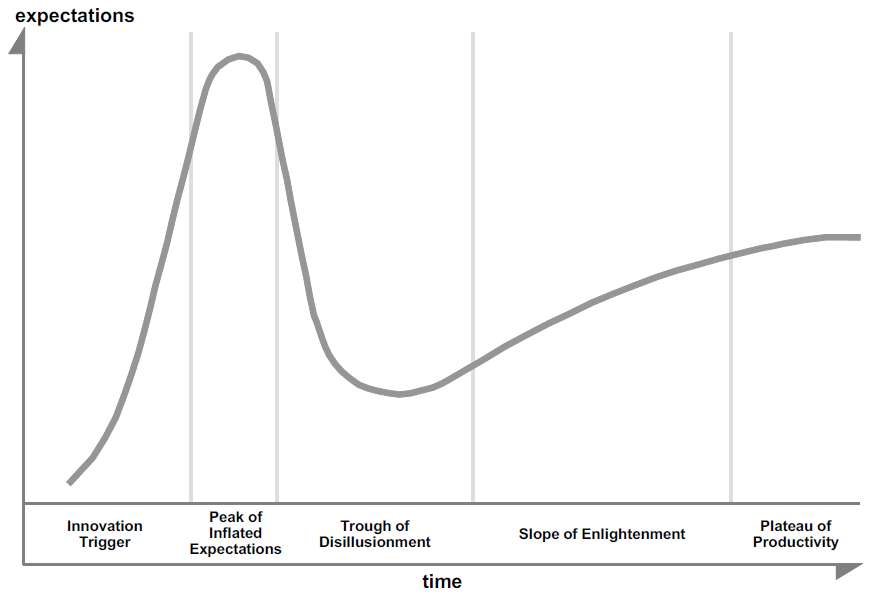
\includegraphics[width=0.9\linewidth]{img/ghc_raw}
	\caption*{\protect\fullciteNP<Quelle:>[S.~4]{Fenn2017}}
	\label{fig:ghc_raw}
\end{figure}

Anhand der Suchergebnisse wird jeder Technologie eine Matrix mit Suchmaschine, Jahr und Anzahl an Treffern zugeordnet. 

Der Betrachtungszeitraum für die Suche erstreckt sich über das Jahr des ersten Erscheinens einer der Technologien aus dem Abschnitt "`Peak of Inflated Expectations"' des "`Gartner Hype Cycle"' bis zum aktuellen Jahr. Das heißt, dass für die Ermittlung des Startjahres alle "`Hype Cycles"' der vergangenen Jahre in die Betrachtung einfließen, so lange mindestens eine der aktuellen Technologien im Abschnitt "`Peak of Inflated Expectations"' darin enthalten ist.

Alternativ kann das erstmalige Erscheinen einer Technologie im Abschnitt "`Innovation Trigger"' als Startzeitpunkt gewählt werden, sofern die Datenmenge im ersten Fall zu gering ausfällt.

Die ermittelte Verteilung der Mengen wird anschließend zunächst pro Suchmaschine und dann kumuliert betrachtet. Die dabei entstandene Kurve der Trefferanzahl über die Zeit wird dazu verwendet, die im Abschnitt "`Peak of Inflated Expectations"' erschienenen Technologien hinsichtlich des Trendverlaufes gegenüberzustellen.
	\section{Technologietrends in der praktizierenden Wirtschaft}

\subsection{Sicht auf Technologien}
Der Begriff Technologie lässt sich als eine spezielle Form des Wissens abstrahieren und entsteht dort, wo dieses Fachwissen Anwendung findet. Deshalb wird sie eher als ihre physikalische Ausprägung wie etwa in Form von Produkten und Systemen wahrgenommen.\footnote{\citeNP<Vgl.>[S.~6f]{Phaal2004}.} Da somit die Aneignung des theoretischen Wissens mit ihrer Implementierung in die Praxis zusammentrifft, ist die Entwicklung neuer Technologien mit verschiedenen Kosten verbunden.

Unternehmen bewegen sich deshalb in einem Spannungsfeld zwischen Investitionen in neue Technologien, um wettbewerbsfähig zu bleiben und optimaler Auslastung ihrer Ressourcenkapazitäten für bestehende Projekte. Denn die Erfolg versprechendste Technologie ist wirkungslos, wenn sie nicht zu einer geeigneten Zeit und mit richtigen Methoden eingesetzt wird.\footnote{\citeNP<Vgl.>[S.~518]{Dickinson2001}.}

Unter dem Begriff F\&E (Forschung und Entwicklung) werden die dafür notwendigen Maßnahmen bezeichnet, die strukturiert in einem Unternehmen gesteuert werden und die Gewinnung neuen Wissens im Bezug auf Technologien als Ziel verfolgen. Dazu werden Ressourcen des Unternehmens, wie etwa Mitarbeiter, monetäre Mittel etc. bereitgestellt, die zunächst einmal keinen unmittelbaren Ertrag herbeiführen, jedoch für die strategische Planung einen wichtigen Beitrag liefern. Ebenso werden Erkenntnisse über die unternehmenseigenen Stärken und Schwächen sowie externe Einflüsse des Marktes in Form von Chancen und Risiken gewonnen.\footnote{\citeNP<Vgl.>[S.~383f]{Jolly2003}.} Es handelt sich somit um eine Management-Tätigkeit, welche unter ständiger Berücksichtigung der Unternehmensziele die Gewinnung, Nutzung und den Schutz von Wissen anstrebt.

Nach Porter gehören F\&E deshalb zu den unterstützenden und nicht zu den primären Aktivitäten der Wertschöpfungskette. Dennoch hält er Technologien innerhalb eines Unternehmens für allgegenwärtig, also mehr oder weniger aller Aktivitäten inhärent. Sie erstrecken sich darüber hinaus auf Lieferanten, Kunden und die Vertriebspolitik, weshalb er hierfür den breiter gefassten Begriff Technologieentwicklung vorzieht.\footnote{\citeNP<Vgl.>[S.~36--42]{Porter1985}.}

Als Unterstützung für den Entscheidungsprozess, welche Technologien potentiell wertvoll im Sinne der Wettbewerbsfähigkeit sind und mit welchen Mitteln die Technologieentwicklung stattfinden sollte, wurden bereits in den 1980er-Jahren Konzepte für das Portfoliomanagement von Technologien entwickelt. Sie sollen die begrenzten Ressourcen eines Unternehmens ausgerichtet an Risiken, Erträgen und der Unternehmensstrategie effizient verteilen.\footnote{\citeNP<Vgl.>[S.~383f]{Jolly2003}.} 

Die wichtigsten Kriterien für die Auswahl der zu untersuchenden bzw. einzusetzenden Technologien ergeben sich aus der Auswertung beeinflussbarer und unbeeinflussbarer Faktoren. Bei den ersteren handelt es sich um firmenspezifische Merkmale sowie den Umgang mit der Wettbewerbssituation.\footnote{\citeNP<Vgl.>[S.~188]{Sinha2005}.} Die Fachkompetenz der Mitarbeiter kann beispielsweise durch Fortbildungen beeinflusst werden. Ebenso obliegt die Entscheidung über strategische Maßnahmen zur Konkurrenzabwehr in der eigenen Hand. Bei den unbeeinflussbaren Faktoren spielt vor allem die Marktsituation eine Rolle. Zum Beispiel ist in schnell wachsenden Marktsegmenten mit einer Vielzahl an Konkurrenten der Zugzwang Alleinstellungsmerkmale zu schaffen durch den Markt vorgegeben. Auch politische Entscheidungen, die direkt oder indirekt auf das eigene Handeln einwirken, liegen in der Regel nicht im Entscheidungsfreiraum eines Unternehmens.\footnote{\citeNP<Vgl.>[S.~188f]{Sinha2005}.}

Aus der Auswertung dieser Kriterien resultiert eine Tendenz, die genauere Prognosen für den optimalen Zeitpunkt des möglichen Einsatzes einer Technologie zulässt.\footnote{\citeNP<Vgl.>[S.~519]{Dickinson2001}.} Basierend darauf können im Hinblick auf potentielle Risiken und Gewinne Investitionen getätigt werden.\footnote{\citeNP<Vgl.>[S.~804]{Dolci2014}.}

\subsection{Einflussfaktoren auf Technologietrends}
Nach Worlton durchlaufen Technologietrends üblicherweise vier Phasen bis zur Marktreife: Erfindung, Innovation, Verschmelzung und Verbreitung. In der ersten Phase wird neues Wissen oder ein neues technisches Instrument generiert bzw. entwickelt. Die Erfindung allein ist dann allerdings in den meisten Fällen noch nicht marktreif, da der konkrete praktische Nutzen hier noch unbekannt ist. Dieser wird während der Innovationsphase durch Iterationen von Versuch und Irrtum in Ansätzen ermittelt. In Phase drei, der Verschmelzung, folgt erst der Durchbruch, indem verschiedene Technologien mit der neuen Erfindung kombiniert werden und ein neues Produkt bilden. Die vollständige Marktreife wird in Phase vier erreicht, wenn das neue Produkt in Stückzahlen produziert werden kann, die der Markt anfragt.\footnote{\citeNP<Vgl.>[S.~313]{Worlton1988}.}

In der wissenschaftlichen Literatur gibt es unterschiedliche Theorien über die treibende Kraft der Technologieentwicklung. Dabei sind zwei herrschende Meinungen festzustellen. Die erste besagt, dass Technologietrends durch äußere Einflüsse, wie den Verbraucher oder Anforderungen des Marktes geprägt werden. Demgegenüber lautet die zweite Annahme, dass der Anbieter im Rahmen seiner Kompetenzen und seines Einsatzes von F\&E Technologietrends ausschlaggebend vorgibt.\footnote{\citeNP<Vgl.>[S.~611]{Adner2001}.}

Adomavicius et al. zufolge ist eine monokausale Betrachtung für die Prognose von Technologietrends nicht zielführend, da sie die Ursachen trivialisiert, die Komplexität bei der Analyse aber nicht reduziert. Sie bevorzugen die Betrachtung von Technologien in einem Ökosystem, wo sie geboren werden, sich von da an stets gegenseitig beeinflussen, folglich einen evolutionären Entwicklungsprozess durchlaufen und wieder verschwinden können. Um die Komplexität der Technologielandschaft zu verringern, widmet er sich technischen Korrelationen zwischen verschiedenen Technologien, anstatt die äußeren Einflüsse Angebot und Nachfrage als alleinigen Impulsgeber zu verstehen.\footnote{\citeNP<Vgl.>[S.~785]{Adovamicius2016}.}

Um das Muster der Technologieentwicklung nachzuvollziehen, ist eine Unterteilung in folgende Rollen hilfreich:\footnote{\citeNP<Vgl.>[S.~786]{Adovamicius2016}.}
\begin{description}
	\item[Komponenten:] Teilstücke von Technologien, die kombiniert ein Produkt bilden.
	\item[Produkte:] Zusammengesetzte Komponenten, die mit dem Anwender interagieren.
	\item[Infrastruktur:] Unterstützen und erweitern die Nutzung eines Produktes.
\end{description}

In Tabelle \ref{tab:influence_path} sind die möglichen Kombinationen von Einflüssen vorhandener in Richtung zukünftiger Technologien abgebildet.

\begin{center}
\captionof{table}{Korrelation der Beeinflussung im technologischen Ökosystem}
\label{tab:influence_path}
\begin{tabulary}{\textwidth}{|L|C|C|C|}
	\hline
	 & zukünftige Komponente & zukünftiges Produkt & zukünftige Infrastruktur \\ 
	\hline 
	vorhandene Komponente &  &  &  \\ 
	\hline 
	vorhandenes Produkt &  &  &  \\ 
	\hline 
	vorhandene Infrastruktur &  &  &  \\ 
	\hline 
\end{tabulary}\par
\bigskip
\bigskip
Quelle: \citeNP<In Anlehnung an>[S.~785]{Adovamicius2016}.
\end{center}


%innovation process
%
%
%technology ecosystem
%Technology driven markets
%process-data-related, sensemaking
%
%Time to market
%
%Standards

\subsection{Informationsquellen von Unternehmern}
Gartner, Forrester, Aberdeen, and IDC

\subsection{Gartner’s Hype Cycle for Emerging Technologies}

\subsection{Schnittpunkte zur akademischen Forschung}
science-to-business
	\section{Technologietrends in der akademischen Forschung}
\subsection{Wissenschaftliche Fachzeitschriften}
Wissenschaftliche Publikationen sind für die Kommunikation und Verbreitung wissenschaftlicher Forschungsergebnisse von essenzieller Bedeutung und leisten einen wesentlichen Beitrag zum Erfolg des Forschenden.\footnote{\citeNP<Vgl.>[S.~417.]{Turbek2016}}

Sie werden hauptsächlich in regelmäßig erscheinenden wissenschaftlichen Fachzeitschriften veröffentlicht, in der Regel in englischer Sprache über einen Drittverlag und nicht der Universität des Autors.\footnote{\citeNP<Vgl.>[o. S.]{Bjork2009}} Zuvor wird ein \glqq Peer-Review\grqq~durch unabhängige Gutachter des gleichen Fachgebietes durchgeführt, bei dem die Qualität und Gültigkeit der Arbeit überprüft werden.\footnote{\citeNP<Vgl.>[S.~707.]{Thurner2011}}

Auch hinsichtlich Form, Umfang, Zitierweise und Schreibstil folgen sie meist bewährten Konventionen.\footnote{\citeNP<Vgl.>[o. S.]{Bjork2009}}

Einer Hochrechnung von \shortciteauthor{Jinha2010} zufolge wurden zwischen der ersten Veröffentlichung eines wissenschaftlichen Artikels im Jahre 1665 in Frankreich und dem Jahr der Studie 2009 insgesamt rund 50 Millionen Forschungsergebnisse nach einem \glqq Peer-Review\grqq~in wissenschaftlichen Artikeln publiziert. Die Verteilung der Publikationen über den analysierten Zeitraum zeigt dabei ein exponentielles Wachstum.\footnote{\citeNP<Vgl.>[S.~261f.]{Jinha2010}}

Im Zeitalter des Internets sind wissenschaftliche Publikationen meist in digitaler Form verfügbar, obgleich der überwiegende Anteil für die Allgemeinheit kostenpflichtig ist.\footnote{\citeNP<Vgl.>[o. S.]{Bjork2009}} Die Entwicklung von wissenschaftlichen Datenbanken schon in der frühen Phase des Internets zeigt, wie wichtig die Speicherung und Verbreitung von Forschungsergebnissen für die Wissenschaft ist.\footnote{\citeNP<Vgl.>[S.~338.]{Falagas2007}}

Sie bieten erweiterte Funktionen zur Suche und Bibliometrie von Artikeln, und werden daher bei der Literaturrecherche ausgiebig eingesetzt, um bereits existierende Forschungsergebnisse auszuwerten. \footnote{\citeNP<Vgl.>[S.~1320.]{Archambault2009}}

\subsection{Bedeutung von Publikationen für die Forschung}
Die Verbreitung von Wissen, das mittels akademischer Forschung gewonnenen wurde, erfolgt hauptsächlich über zwei Kanäle: Lehre und Publikationen in wissenschaftlichen Zeitschriften. Letzterer gewinnt dabei immer mehr an Bedeutung, da er vor allem für Forscher, die am Anfang ihrer Laufbahn stehen, bessere Möglichkeiten für ihre Karriere bietet.\footnote{\citeNP<Vgl.>[S.~322f.]{DeRond2005}}

Der Aphorismus \glqq Publish or Perish\grqq\footnote{Englisch sinngemäß für \glqq Publizieren oder Untergehen\grqq.} verdeutlicht den Druck, der auf Wissenschaftlern lastet, relevante Forschungsergebnisse in renommierten Fachzeitschriften zu veröffentlichen, um die nötige Aufmerksamkeit auf die eigenen Fähigkeiten zu lenken und damit die Karriereoptionen zu verbessern.\footnote{\citeNP<Vgl.>[S.~391.]{Clapham2005}}

Eine kontinuierliche Veröffentlichung von Forschungsergebnissen kann auch für Unternehmen nützlich sein, da Innovationen, die von Wettbewerbern parallel entwickelt und patentiert werden, rechtlich weiterhin nutzbar bleiben.\footnote{\citeNP<Vgl.>[S.~927.]{Parchomovsky2000}}

\subsection{Trends in der akademischen Forschung}
Forschungstrends in der wissenschaftlichen Fachliteratur können sowohl interne als auch externe Ursachen haben. Typische interne Ursachen sind neue Entdeckungen und wissenschaftliche Durchbrüche durch andere Forscher, die erhöhte Forschungspotentiale auslösen können. Externe Ursachen sind natürliche bzw. gesellschaftliche Ereignisse, die unabhängig von der Forschung eintreten und Wissenschaftler dazu anregen können, ein Thema aus neuen Perspektiven zu untersuchen.\footnote{\citeNP<Vgl.>[S.~359.]{Chen2006}}

Bei den internen Ursachen sind kontinuierliche Verbesserungen an bestehenden Technologien von revolutionär neuen Technologien zu unterscheiden.\footnote{\citeNP<Vgl.>[S.~114.]{Dotsika2017}} Letztere haben weitreichendere Auswirkungen auf das sozioökonomische System und werden in der Literatur oft als \glqq Emerging Technologies\grqq~bzw. \glqq Disruptive Technologies\grqq~bezeichnet.\footnote{\citeNP<Vgl.>[S.~285.]{Li2018}} Der Unterschied besteht in der anwendungsorientierten Reife der neuen Technologie. Bei einer \glqq Emerging Technology\grqq~muss der praktische Nutzen einer theoretischen Erkenntnis zunächst festgestellt werden. Die sog. \glqq Disruptive Technology\grqq~hat diese Phase bereits durch eine signifikante finanzielle oder technologische Verbesserung positiv gemeistert.\footnote{\citeNP<Vgl.>[S.~294.]{Li2018}}

Diese Art von Technologien haben einen potentiell stärkeren Effekt auf Forschungstrends in der Wissenschaft als solche, die auf Basis vorhandener Technologien mit marginalen Verbesserungen ausgestattet wurden.

\shortciteauthor{Price1965} zufolge kann ein Muster für Forschungsschwerpunkte zu einem bestimmten Thema beobachtet werden. Neue wissenschaftliche Artikel beziehen sich demnach eher auf die aktuellsten Publikationen als auf deren Vorgänger. Im Umkehrschluss bedeutet das, dass die meist zitierten Artikel gleichzeitig auch die aktuellsten sind.\footnote{\citeNP<Vgl.>[S.~512f.]{Price1965}} Dieser Effekt gibt eine gute Erklärung für das bekannte Phänomen, dass Artikel wenige Jahre nach ihrer Veröffentlichung als veraltet gelten.\footnote{\citeNP<Vgl.>[S.~360.]{Chen2006}}

\subsection{Schnittstellen mit der praktizierenden Wirtschaft}
Da die öffentlichen Mittel für die akademische Forschung heute nicht wesentlich zunehmen, wird die industrielle Zusammenarbeit von vielen Wissenschaftlern als eine Strategie angesehen, um mehr finanzielle Unterstützung für ihre Forschung zu erhalten.\footnote{\citeNP<Vgl.>[S.~86.]{Calvert2003}}
	\section{Methodische Vorgehensweise}
\subsection{Datenerhebung}
Für die Gegenüberstellung der Technologietrends in der akademischen Forschung und praktizierenden Wirtschaft werden, wie bereits in Abschnitt \ref{sec:method} erwähnt, zwei Arten von Quellen herangezogen.

Der \glqq Gartner Hype Cycle for Emerging Technologies\grqq~repräsentiert als marktführendes Unternehmen für Technologieprognosen den Part der praktizierenden Wirtschaft. Dabei dienen die Technologien im Bereich der \glqq Peak of Inflated Expectations\grqq~in vorliegender Gewichtung als Datenbasis für die Analyse.

Demgegenüber wird die Datenbasis der akademischen Forschung aus Abfragen in relevanten Literaturdatenbanken erhoben. 

\subsection{Operationalisierung der Daten}
\subsection{Methodik der Analyse}
	\section{Ergebnisse der Untersuchung}
Im nächsten Schritt gilt es, einen Eindruck über die Verteilung der Daten im Hinblick auf die Beantwortung der Leitfragen zu gewinnen. Dazu werden sie zunächst einmal adäquat gruppiert und in einem Graphen geplottet.

\subsection{Trendverlauf im \glqq Hype Cyle\grqq}
Die Verteilung der Technologien aus dem Jahre 2016 über alle Veröffentlichungen ist in Abbildung \ref{fig:ghc_trend} zu sehen. Das zum Plotten der Graphik verwendete R-Skript ist in Anhang \ref{sec:ghc_trend_plot} zu finden.

\begin{figure}
	\centering
	\caption{Trendverlauf der Technologien aus dem \glqq Gartner Hype Cycle\grqq}
	\includegraphics[width=\linewidth,clip,trim=0cm 0.5cm 1cm 2cm]{pdf/ghc_trend.pdf}
	\caption*{Quelle: Eigene Darstellung}
	\label{fig:ghc_trend}
\end{figure}

Die Legende listet die Symbole und dazugehörigen Farben zu den abgekürzten Technologien auf, mit denen die Koordinatenpunkte markiert sind. Insgesamt sind elf Technologien über den Zeitraum von 2010 bis 2017 abgebildet. Die Reihenfolge der Auflistung ergibt sich aus der Reihung der ursprünglichen Ausgabe.

Zunächst einmal fällt auf, dass sich die Technologien des ausgewählten Zeitraumes relativ eng um das Jahr der Vergleichsbasis befinden. Die Standardabweichung beträgt aufgerundet gerade einmal 1,8 um das Veröffentlichungsjahr 2016.

Einzig die Trendtechnologie \glqq Autonomous Verhicles\grqq~erstreckt sich, mit einer Unterbrechung im Jahre 2011, über den gesamten Zeitraum. Im Jahre 2014 steigt sie aus der Phase \glqq Innovation Trigger\grqq~in die Phase \glqq Peak of Inflated Expectations\grqq~auf und ist seitdem dort vertreten. Im Jahre 2015 erreicht sie ihre Höchstform als stärkster Trend des Jahres.

Die Technologien \glqq Smart Robots\grqq~und \glqq Connected Home\grqq~erscheinen erstmalig im Jahre 2014 im \glqq Innovation Trigger\grqq~und sind seit 2016 in den \glqq Peak of Inflated Expectations\grqq~aufgestiegen.

Im Jahr darauf erscheinen zwei der Technologien, \glqq Micro Data Centers\grqq~und \glqq Machine Learning\grqq~initial im \glqq Peak of Inflated Expectations\grqq~sowie \glqq Software-Defined Security\grqq~in der Phase \glqq Innovation Trigger\grqq. Die Technologie \glqq Micro Data Centers\grqq~verbleibt im Folgejahr auf vergleichbarem Niveau und fällt im Jahre 2017 aus dem \glqq Hype Cycle\grqq~heraus. \glqq Machine Learning\grqq~hingegen verbleibt bis zur letzten Ausgabe in der gleichen Phase auf höchstem Trendniveau, im Jahre 2016 erreicht sie sogar den höchsten Punkt der Trendkurve. \glqq Software-Defined Security\grqq~erfährt wiederum eine relativ schnelle Reife\-entwicklung. Im Jahre 2016 ist sie bereits im \glqq Peak of Inflated Expectations\grqq~und wieder ein Jahr später im \glqq Trough of Disillusionment\grqq. Damit ist sie die einzige Technologie aus der Datenbasis die alle drei Phasen unmittelbar aufeinanderfolgend belegt.

Da es sich um die Datenbasis handelt, sind alle übrigen Technologien im Jahr 2016 erstmalig in Erscheinung getreten und befinden sich im Abschnitt \glqq Peak of Inflated Expectations\grqq. \glqq Gesture Control Devices\grqq~und \glqq Software-Defined Anything\grqq~sind bereits im darauffolgenden Jahr nicht mehr im \glqq Hype Cycle\grqq. \glqq Blockchain\grqq~und \glqq Nanotube Electronics\grqq~hingegen befinden sich auch in der aktuellsten Ausgabe im \glqq Peak of Inflated Expectations\grqq~und \glqq Cognitive Expert Advisors\grqq~schließlich ist zum gleichen Zeitpunkt eine Ebene höher gekommen, in die Phase \glqq Trough of Disillusionment\grqq.

Für die Leitfrage L2 ist das Jahr der ersten Veröffentlichung einer Technologie im \glqq Hype Cycle\grqq~von Bedeutung. Diese werden in Tabelle \ref{tab:ghc_init} festgehalten.

\begin{table}
	\caption{Erstmaliges Erscheinungsjahr der Technologien im \glqq Gartner Hype Cycle\grqq}
	\fontfamily{pcr}\selectfont
	\centering
	\label{tab:ghc_init}
	\begin{tabularx}{\linewidth}{X|p{3em}XXX}
	Erst\-erscheinung & 2010 & 2014 & 2015 & 2016 \\
	\hline
	Technologien & \acs{AV} & \acs{SR}, \acs{CH} & \acs{MDC}, \acs{ML}, \acs{SDS} & \acs{GCD}, \acs{B}, \acs{CEA}, \acs{NE}, \acs{SDx} \\
	\end{tabularx}
	\caption*{Quelle: Eigene Darstellung}
\end{table}

Für die Beantwortung der Leitfrage L3 werden die Technologien benötigt, die nach Erscheinen in einer Ausgabe des \glqq Hype Cycle\grqq~im Folgejahr weggefallen sind. Die Technologien und das Jahr der Absenz werden deshalb in Tabelle \ref{tab:ghc_abscence} zusammengefasst.

\begin{table}
	\caption{Veröffentlichungsjahre der Absenz von Technologien im \glqq Gartner Hype Cycle\grqq}
	\fontfamily{pcr}\selectfont
	\centering
	\label{tab:ghc_abscence}
	\begin{tabularx}{\linewidth}{X|XX}
		Absenzjahr & 2011 & 2017  \\
		\hline
		Technologien & \acs{AV} & \acs{GCD}, \acs{MDC}, \acs{SDx} \\
	\end{tabularx}
	\caption*{Quelle: Eigene Darstellung}
\end{table}

\subsection{Trendverlauf in der akademischen Forschung}
Die Bestimmung des Trendverlaufes in der akademischen Forschung ist umfangreicher als im \glqq Hype Cycle\grqq. Dies basiert auf der Möglichkeit, die wissenschaftlichen Publikationen im Hinblick auf den Trendverlauf genauer auswerten zu können, da die auswertbaren Parameter breiter gefächert sind.

Zunächst einmal werden unterschiedliche Datenquellen für die Ermittlung der Trend\-stär\-ke eingesetzt, was im Ge\-gen\-satz zum \glqq Hype Cycle\grqq~eine Er\-hö\-hung der Datenmenge herbeiführt. Auch die Unterteilung in unterschiedliche Veröffentlichungstypen erhöht die notwendigen Aktionen für das Visualisieren und Auswerten. Auf der anderen Seite ist durch die Möglichkeit, konkrete Veröffentlichungsmengen zu bestimmen, eine genauere Analyse möglich und nötig.

Wegen der Unterteilung in verschiedene Veröffentlichungstypen, ist sowohl der differenzierte, relative Trend, wie die kumulierte Gesamtmenge der Publikationen zu betrachten.

Im Folgenden wird die Mengenverteilung der Veröffentlichungen zu den einzelnen Technologien betrachtet. Pro Suchmaschine und Veröffentlichungstyp ist jeweils eine Kurve abgebildet. Dies wird durch unterschiedliche Linientypen und Punktsymbole kenntlich gemacht.

In Abbildung \ref{fig:gcd_pub} ist die Verteilung der Veröffentlichungen zur Technologie \glqq Gesture Control Devices\grqq~dargestellt. Es ist festzustellen, dass die absoluten Mengen an Publikationen im Verhältnis zu den Gesamtveröffentlichungen in Tabelle \ref{tab:dist_full_pub} trotz Erweiterung des Suchbegriffes mit weit unter 0,1~\% sehr gering Ausfallen. Der relative Trend zeigt eine Ansammlung bei steigender Tendenz im Jahre 2016 für vier von sechs Kurven. Konferenzbeiträge im \ac{ACM} kommen am häufigsten vor und haben ihren Höhepunkt in den Jahren 2013 und 2014 mit rund doppelt so viel Publikationen wie Konferenzbeiträge bei \ac{IEEE}. Konferenzbeiträge im \ac{WoS} sowie Artikel im \ac{IEEE} kommen vernachlässigbar wenig vor.

\begin{figure}
	\centering
	\caption{Verteilung von Publikationen zu \glqq Gesture Control Devices\grqq}
	\includegraphics[width=\linewidth,clip,trim=0cm 0.5cm 1cm 0.8cm,height=90mm]{pdf/GCD.pdf}
	\caption*{Quelle: Eigene Darstellung}
	\label{fig:gcd_pub}
\end{figure}

Abbildung \ref{fig:mdc_pub} zeigt die entsprechende Graphik zu \glqq \acl{MDC}\grqq. Der Suchbegriff wurde nur um verschiedene Schreibweisen der Technologie erweitert. Die absoluten Häufigkeiten sind noch geringer als die der vorhergehenden Technologie. Konferenzberichte im \ac{WoS} sind nicht vorhanden. Die ersten Publikationen überhaupt sind im Jahre 2011 als Konferenzberichte im \ac{ACM} erschienen. Der relative Trend hingegen liegt auch im Jahre 2016.

\begin{figure}
	\centering
	\caption{Verteilung von Publikationen zu \glqq \acl{MDC}\grqq}
	\includegraphics[width=\linewidth,clip,trim=0cm 0.5cm 1cm 0.8cm,height=90mm]{pdf/MDC.pdf}
	\caption*{Quelle: Eigene Darstellung}
	\label{fig:mdc_pub}
\end{figure}

Der Verlauf von \glqq Smart Robots\grqq~ist in Abbildung \ref{fig:sr_pub} zu sehen. Der Begriff wurde um die unterschiedlichen Bezeichnungen in der Literatur ergänzt. Die Technologie ist im gesamten Betrachtungszeitraum und darüber hinaus in der wissenschaftlichen Literatur vertreten. Eine signifikante Anzahl an Publikationen ist in Konferenzbeiträgen im \ac{IEEE} zu verzeichnen, die mit \numprint{1320} Publikationen ihren Höhepunkt erneut im Jahre 2016 erreichen. Auch wenn sie mit knapp 300 publizierten Fachartikeln deutlich darunter liegen, ist diese Menge bereits größer als zu den bisherigen Technologien. Von 2014 bis 2017 ist die Anzahl an Publikationen stets höher als im Vorjahr. Die übrigen Veröffentlichungen sind im Verhältnis dazu relativ niedrig.

Alles in allem lässt sich sagen, dass die Technologie \glqq Smart Robots\grqq~ein erhöhtes Maß an Aufmerksamkeit in der Wissenschaft im Vergleich zu den bisherigen Technologien erlangt hat.

\begin{figure}
	\centering
	\caption{Verteilung von Publikationen zu \glqq Smart Robots\grqq}
	\includegraphics[width=\linewidth,clip,trim=0cm 0.5cm 1cm 0.8cm,height=90mm]{pdf/SR.pdf}
	\caption*{Quelle: Eigene Darstellung}
	\label{fig:sr_pub}
\end{figure}

Die ersten nennenswerten Publikationen zur \glqq Blockchain-Technologie\grqq, deren Publikationsverlauf in Abbildung \ref{fig:b_pub} abgebildet ist, sind erst im Jahre 2016 zu verzeichnen. Um die 50 Publikationen sind jeweils in Fachartikeln im \ac{WoS} sowie Konferenzbeiträgen im \ac{IEEE} und \ac{ACM} erschienen. Im Jahr darauf steigen alle Veröffentlichungsformen -- bis auf Konferenzbeiträge im \ac{WoS} -- steil an, sodass die ersten drei Kurven ihre Anzahl im Vergleich zum Vorjahr mindestens verdoppeln.

\begin{figure}
	\centering
	\caption{Verteilung von Publikationen zu \glqq Blockchain\grqq}
	\includegraphics[width=\linewidth,clip,trim=0cm 0.5cm 1cm 0.8cm,height=90mm]{pdf/B.pdf}
	\caption*{Quelle: Eigene Darstellung}
	\label{fig:b_pub}
\end{figure}

\glqq Connected Home\grqq~gehört ebenfalls zu den Technologien, die in der Wissenschaft eine gewisse Beachtung finden. In Abbildung \ref{fig:ch_pub} ist zu erkennen, dass schon zu Beginn des Betrachtungszeitraumes bei \ac{IEEE} und \ac{ACM} mit etwa 150 Konferenzbeiträgen ein relativ hohes Interesse an der Technologie vorhanden ist. Die Tendenz an Publikationen ist, ausgenommen von Konferenzbeiträgen im \ac{ACM}, bis 2017 steigend. Sie erreicht ihren Höhepunkt im Jahre 2017 und liegt für Konferenzbeiträge im \ac{IEEE} und Fachartikel im \ac{WoS} bei ca. 400 Veröffentlichungen. Dazu war es allerdings notwendig, den Technologiebegriff bei der Suche um die gängigen Synonyme zu erweitern.

\begin{figure}
	\centering
	\caption{Verteilung von Publikationen zu \glqq Connected Home\grqq}
	\includegraphics[width=\linewidth,clip,trim=0cm 0.5cm 1cm 0.8cm,height=90mm]{pdf/CH.pdf}
	\caption*{Quelle: Eigene Darstellung}
	\label{fig:ch_pub}
\end{figure}

Als nächstes ist die Technologie \glqq Cognitive Expert Advisors\grqq~in Abbildung \ref{fig:cea_pub} zu sehen, die offenbar ebenso zu den bedeutenderen Technologien aus wissenschaftlicher Perspektive gehört. Sie erreicht zeitweise um die \numprint{1500} Fachartikel im \ac{ACM}, allerdings mit einer fallenden Tendenz, welche jedoch nicht unter 500 fällt. Konferenzbeiträge im \ac{IEEE} sowie Fachartikel im \ac{WoS} liegen im Betrachtungszeitraum relativ konstant bei ca. 500 Veröffentlichungen. Die anderen sind aktuell eher unbedeutend.

\begin{figure}
\centering
\caption{Verteilung von Publikationen zu \glqq Cognitive Expert Advisors\grqq}
\includegraphics[width=\linewidth,clip,trim=0cm 0.5cm 1cm 0.8cm,height=90mm]{pdf/CEA.pdf}
\caption*{Quelle: Eigene Darstellung}
\label{fig:cea_pub}
\end{figure}

Die Technologie \glqq \acl{ML}\grqq~hat mit Abstand die höchsten Publikationszahlen unter den untersuchten Technologien. Die Trends in den einzelnen Ausprägungen von Publikationen sind jedoch unterschiedlich. Abbildung \ref{fig:ml_pub} zeigt, dass Konferenzbeiträge im \ac{IEEE} sowie Fachartikel im \ac{WoS} im Betrachtungszeitraum ein starkes positives Wachstum erfahren und von 2014 an nahezu parallel und in Tausenderschritten die Anzahl von über \numprint{5000} Publikationen erreichen. Beide Veröffentlichungstypen im \ac{ACM} pendeln sich ab 2016 bei ca. \numprint{1000} Veröffentlichungen ein. Fachartikel im \ac{IEEE} hingegen erreichen eine Anzahl von ungefähr 800 im Jahre 2017 nach zuvor mäßigem Wachstum. Allein die Konferenzbeiträge im \ac{WoS} fallen -- absolut betrachtet -- auffallend gering aus. Doch auch hier handelt es sich um die höchsten Werte über alle Konferenzbeiträge im \ac{WoS}. Dabei wurde die durch Ausschluss der Nachfolgetechnologie \glqq Deep Learning\grqq~eingeschränkt.

\begin{figure}
	\centering
	\caption{Verteilung von Publikationen zu \glqq Machine Learning\grqq}
	\includegraphics[width=\linewidth,clip,trim=0cm 0.5cm 1cm 0.8cm,height=90mm]{pdf/ML.pdf}
	\caption*{Quelle: Eigene Darstellung}
	\label{fig:ml_pub}
\end{figure}

Abbildung \ref{fig:sds_pub} stellt den Verlauf der Technologie \glqq Software-Defined Security\grqq~dar. Die Publikationen dazu sind marginal. Einzig nennenswert ist die steigende Tendenz für Konferenzbeiträge im \ac{IEEE}, die allerdings mit zehn Publikationen in 2017 schon den Höchstwert ausmacht.

\begin{figure}
	\centering
	\caption{Verteilung von Publikationen zu \glqq Software-Defined Security\grqq}
	\includegraphics[width=\linewidth,clip,trim=0cm 0.5cm 1cm 0.8cm,height=90mm]{pdf/SDS.pdf}
	\caption*{Quelle: Eigene Darstellung}
	\label{fig:sds_pub}
\end{figure}

Der Trendverlauf der Technologie \glqq Autonomous Vehicles\grqq~ist Abbildung \ref{fig:av_pub} zu entnehmen. Erneut heben sich die Kurven der Konferenzberichte im \ac{IEEE} und Fachartikel im \ac{WoS} den anderen gegenüber ab. Erstere steigen ab 2015 stärker an als in den Jahren davor und kommen in 2017 auf 675 Veröffentlichungen. Die Fachartikel im \ac{WoS} kommen auf 361 im selben Jahr. Konferenzberichte im \ac{WoS} sind auch hier kaum vorhanden. Die anderen Veröffentlichungen bewegen sich mit leicht steigender Tendenz um die Anzahl von 100 herum.

\begin{figure}
	\centering
	\caption{Verteilung von Publikationen zu \glqq Autonomous Vehicles\grqq}
	\includegraphics[width=\linewidth,clip,trim=0cm 0.5cm 1cm 0.8cm,height=90mm]{pdf/AV.pdf}
	\caption*{Quelle: Eigene Darstellung}
	\label{fig:av_pub}
\end{figure}

Schließlich zeigt Abbildung \ref{fig:ne_pub} die Trendentwicklung der Technologie \glqq Nanotube Electronics\grqq. Erneut ist zu sehen, dass Konferenzberichte im \ac{IEEE} und Fachartikel im \ac{WoS} die übrigen Publikationen dominieren. Sie bewegen sich im Betrachtungszeitraum um 100 Publikationen herum, allerdings mit einer leicht fallenden Tendenz. Im Jahre 2016 ist ein leichter Ausschlag nach oben zu erkennen. Konferenzberichte im \ac{WoS} sind wieder kaum vorhanden. Der Rest befindet sich relativ konstant bei um die 20 Veröffentlichungen.

\begin{figure}
	\centering
	\caption{Verteilung von Publikationen zu \glqq Nanotube Electronics\grqq}
	\includegraphics[width=\linewidth,clip,trim=0cm 0.5cm 1cm 0.8cm,height=90mm]{pdf/NE.pdf}
	\caption*{Quelle: Eigene Darstellung}
	\label{fig:ne_pub}
\end{figure}

Da die Technologie \glqq Software-Defined Anything\grqq~ -- auch über den Betrachtungszeitraum hinaus -- kaum nennenswert in wissenschaftlichen Publikationen vorkommt, wird sie nicht visualisiert.

\subsection{Klassifizierung der Technologien}
Durch die deskriptive Auswertung der Daten sind Muster zu erkennen, die eine Klassifizierung der Technologien ermöglichen. Sie dient der besseren Vergleichbarkeit des Trendverhältnisses zwischen Wirtschaft und Wissenschaft.

In Tabelle \ref{tab:class_trend_ev} sind die Technologien den in Abschnitt \ref{sec:class_tech} definierten Trendstufen zugeordnet. Die zeitliche Verteilung dazu ist in den Zellen durch die Angabe des entsprechenden Zeitraumes bzw.~-punktes abgebildet.

\begin{table}
	\caption{Zeitliche Zuordnung von Technologien zu Trendstufen}
	\fontfamily{pcr}\selectfont
	\footnotesize
	\centering
	\label{tab:class_trend_ev}
	\begin{tabularx}{\linewidth}{p{2.2cm}|XXXXX}
		Technologie & $>$ 2000 & $>$ 500 & $>$ 100 & $>$ 20 & $<$ 20 \\
		\hline
		\acs{GCD} & - & - & 2014 & 2011-2013 2015-2017 & 2010 \\
		\acs{MDC} & - & - & - & - & 2011-2017 \\
		\acs{SR} & - & 2010-2017 & - & - & - \\
		\acs{B} & - & & 2016 & - & 2013-2015 \\
		\acs{CH} & - & 2012-2017 & 2010-2011 & - & - \\
		\acs{CEA} & 2010-2012 & 2013-2017 & - & - & - \\
		\acs{ML} & 2010-2017 & - & - & - & - \\
		\acs{SDS} & - & - & - & - & 2014-2017 \\
		\acs{AV} & - & 2015-2017 & 2010-2014 & - & - \\
		\acs{NE} & - & - & 2010-2017 & - & - \\
		\acs{SDx} & - & - & - & - & 2017 \\
		\hline
	\end{tabularx}
	\caption*{Quelle: Eigene Darstellung}
\end{table}

Tabelle \ref{tab:class_tech} zeigt die Zuordnung der Technologien zu ihren Rollen. Bei nicht ganz eindeutigen Zugehörigkeiten bzw. Überschneidungen werden sie der passendsten Kategorie zugewiesen, wodurch eine Eindeutigkeit gewährleistet wird.

\begin{table}
	\caption{Rollenbasierte Klassifizierung der Technologien}
	\fontfamily{pcr}\selectfont
%	\footnotesize
	\centering
	\label{tab:class_tech}
	\begin{tabularx}{\linewidth}{X|XXX}
		Technologie & Produkt & Infrastruktur & Komponente \\
		\hline
		\acs{GCD} & $\checkmark$ & & \\
		\hline
		\acs{MDC} & & $\checkmark$ & \\
		\hline
		\acs{SR} & $\checkmark$ & & \\
		\hline
		\acs{B} & & $\checkmark$ & \\
		\hline
		\acs{CH} & $\checkmark$ & & \\
		\hline
		\acs{CEA} & & & $\checkmark$ \\
		\hline
		\acs{ML} & & & $\checkmark$ \\
		\hline
		\acs{SDS} & & $\checkmark$ & \\
		\hline
		\acs{AV} & $\checkmark$ & & \\
		\hline
		\acs{NE} & & & $\checkmark$ \\
		\hline
		\acs{SDx} & & $\checkmark$ & \\
		\hline
	\end{tabularx}
	\caption*{Quelle: Eigene Darstellung}
\end{table}
	\renewcommand{\appendixname}{Anhang}
\renewcommand{\appendixtocname}{Anhang}
\renewcommand{\appendixpagename}{Anhang}

\begin{appendices}
	\addtocontents{toc}{\protect\setcounter{tocdepth}{0}}
	\section{}\label{sec:sci_raw_dist}
\end{appendices}


%\begin{description}
%	\item[GCD:]	\begin{verbatim}
%	(TS=("natural user interface"
%	OR "gesture control device"
%	OR "gesture control devices"))
%	AND DOCUMENT TYPES: (Article)
%	\end{verbatim}
%	\item[MDC:] \begin{verbatim}(TS=("micro data center"
%	OR "micro data centers"
%	OR "microdata center"
%	OR "microdata centers"
%	OR "micro datacenter"
%	OR "micro datacenters"))
%	AND DOCUMENT TYPES: (Article / Proceedings Paper)\end{verbatim}
%	\item[SR:] \begin{verbatim}(TS=("smart robot"
%	OR "smart robots"
%	OR "cognitive robotics"
%	OR "cognitive robotic"
%	OR "humanoid robot"
%	OR "humanoid robots"
%	OR "android robot"
%	OR "android robots"))
%	AND DOCUMENT TYPES: (Article) \end{verbatim}
%	\item[B:] \begin{verbatim}(TS=("blockchain"))
%	AND DOCUMENT TYPES: (Article)\end{verbatim}
%	\item[CH:] \begin{verbatim}(TS=("connected home"
%	OR "connected homes"
%	OR "smart home"
%	OR "smart homes"))
%	AND DOCUMENT TYPES: (Article)\end{verbatim}
%	\item[CEA:] \begin{verbatim}(TS=("cognitive expert system"
%	OR "cognitive expert systems"
%	OR "cognitive expert advisor"
%	OR "cognitive expert advisors"))
%	AND DOCUMENT TYPES: (Article)\end{verbatim}
%	\item[ML:] \begin{verbatim}(TS=("machine learning"
%	NOT "deep learning"))
%	AND DOCUMENT TYPES: (Article)\end{verbatim}
%	\item[SDS:] \begin{verbatim}(TS=("software defined security"
%	OR "software-defined security"))
%	AND DOCUMENT TYPES: (Article)\end{verbatim}
%	\item[AV:] \begin{verbatim}(TS=("autonomous vehicle"
%	OR "autonomous vehicles"))
%	AND DOCUMENT TYPES: (Article)\end{verbatim}
%	\item[NE:] \begin{verbatim}(TS=("CNTFET"
%	OR "nanotube electronic"
%	OR "nanotube electronics"
%	OR "carbon nanotube field effect"
%	OR "carbon nanotube field-effect"
%	OR "semiconductor nanotubes"))
%	AND DOCUMENT TYPES: (Article)
%	\end{verbatim}
%	\item[SDx:] \begin{verbatim}(TS=("software defined anything"
%	OR "software-defined anything"))
%	AND DOCUMENT TYPES: (Article)\end{verbatim}
%\end{description}

keywords.author.keyword:("natural user interface" "gesture control devices" "gesture control device") OR recordAbstract:("gesture control devices" "gesture control device" "natural user interface") OR acmdlTitle:("gesture control devices" "gesture control device" "natural user interface")

keywords.author.keyword:("micro data center" "micro data centers" "microdata center" "microdata centers" "micro datacenter" "micro datacenters") OR recordAbstract:("micro data center" "micro data centers" "microdata center" "microdata centers" "micro datacenter" "micro datacenters") OR acmdlTitle:("micro data center" "micro data centers" "microdata center" "microdata centers" "micro datacenter" "micro datacenters")

acmdlTitle:("machine learning" -"deep learning") OR recordAbstract:("machine learning" -"deep learning") OR keywords.author.keyword:("machine learning" -"deep learning")

acmdlTitle:(CNTFET "nanotube electronic" "nanotube electronics" "carbon nanotube field effect" "carbon nanotube field-effect" "semiconductor nanotubes") OR recordAbstract:(CNTFET "nanotube electronic" "nanotube electronics" "carbon nanotube field effect" "carbon nanotube field-effect" "semiconductor nanotubes") OR keywords.author.keyword:(CNTFET "nanotube electronic" "nanotube electronics" "carbon nanotube field effect" "carbon nanotube field-effect" "semiconductor nanotubes")


WOS All
(PY=(2018)) AND DOCUMENT TYPES: (Proceedings Paper)

IEEE All
\url{https://ieeexplore.ieee.org/search/searchresult.jsp?refinements=ContentType:Conferences&searchWithin=%22Publication_Year%22:2012}
	
ACM All
\url{https://dl.acm.org/results.cfm?query=%2A&filtered=allPubGroups%2EallPubGroup=Proceeding&within=owners%2Eowner%3DGUIDE&dte=2010&bfr=2010}
	\clearpage
	\addtocontents{toc}{\protect\setcounter{tocdepth}{2}}
	\renewcommand{\refname}{Literaturverzeichnis}
	\pagenumbering{roman}
	\singlespacing
	\bibliography{lit}
	\onehalfspacing
	\newpage
\fancyhead[C]{\thepage}
\pagenumbering{gobble} % Keine Seitenzahlen mehr

%-----------------------------------
% Ehrenwörtliche Erklärung
%-----------------------------------
\section*{Ehrenwörtliche Erklärung}
Hiermit versichere ich, dass die vorliegende Arbeit von mir selbstständig und ohne unerlaubte Hilfe angefertigt worden ist, insbesondere dass ich alle Stellen, die wörtlich oder annähernd wörtlich aus Veröffentlichungen entnommen sind, durch Zitate als solche gekennzeichnet habe. Ich versichere auch, dass die von mir eingereichte schriftliche Version mit der digitalen Version übereinstimmt. Weiterhin erkläre ich, dass die Arbeit in gleicher oder ähnlicher Form noch keiner Prüfungsbehörde / Prüfungsstelle vorgelegen hat. Ich erkläre mich damit einverstanden, dass die Arbeit der Öffentlichkeit zugänglich gemacht wird. Ich erkläre mich damit einverstanden, dass die Digitalversion dieser Arbeit zwecks Plagiatsprüfung auf die Server externer Anbieter hochgeladen werden darf. Die Plagiatsprüfung stellt keine Zurverfügungstellung für die Öffentlichkeit dar.


\vspace{5cm}

\begin{table}[h]
	\centering
	\begin{tabular*}{\textwidth}{c @{\extracolsep{\fill}} ccccc}
		Gelsenkirchen, \today
		&
		%PLACE YOUR SCANNED SIGNATURE INSIDE YOUR PICTURE DIRECTORY. CALL IT unterschrift.jpg
%		
\includegraphics[width=0.35\textwidth]{img/unterschrift}\vspace*{-0.35cm}
		\\
		\rule[0.5ex]{12em}{0.55pt} & \rule[0.5ex]{12em}{0.55pt} \\
		(Ort, Datum) & (Eigenhändige Unterschrift)
		\\
	\end{tabular*} \\
\end{table}

\end{document}